%tukaj zaporedoma napisemo{st. zaporedne ure}{datum}{naslov}{poglavje}{oblika dela}{pripomocki}
\begin{priprava}{}{}{Zaporedja}{Uvod}{frontalna}{tabla}

% Definicija zaporedja

\didopomba{Vprašaš, kaj je zaporedje. Načeloma že itak vejo, kaj je zaporedje -- nekaj si sledi po vrsti, lahko so to števila, črke, simboli itd.}

Zaporedje števil je niz števil, ki si sledijo po vrsti, npr. \didopomba{naj predlagajo sami}
$$ 8, 6, 45, -9, \sqrt{19}, \pi, e^2, i-8 \ldots $$
Vsako število v zaporedju se imenuje \textbf{člen zaporedja}. V splošnem lahko zaporedje zapišemo s simboli:
$$ a_1, a_2, a_3, a_4, a_5, a_6 \ldots, a_n, a_{n+1} \ldots, $$

kjer so $ a_1 $ prvi člen zaporedja, $ a_2 $ drugi člen zaporedja itd.; $ a_n $ imenujemo $n$-ti člen oz. \textbf{splošni člen} zaporedja.

\textbf{Končno} zaporedje ima končno število členov (npr. $ 1, 2, 3, 2, 1 $), \textbf{neskončno} pa neskončno (npr. $ 3, 6, 9, 12, 15 \ldots $).

Nas zanimajo zaporedja, ki jim lahko določimo člene \didopomba{našteješ zaporadja, za vsako najprej vprašaš za naslednje konkretne člene, šele nato za splošni člen}:
\begin{align*}
    & 1, 2, 3, 4, 5, 6 \ldots && a_n = n \\
    & 2, 4, 8, 16, 32 \ldots && a_n = 2^n \\
    & 1, 2, 4, 8, 16, 32 \ldots && a_n = 2^{n-1} \\
    & 4, 7, 10, 13, 16 \ldots && a_n = 3n + 1 \\
    & 1, 1, 2, 3, 5, 8, 13 \ldots && a_n = a_{n-2} + a_{n-1} \text{ (Fibonaccijevo zaporedje)}
\end{align*}

\textbf{Zaporedje realnih števil je predpis, ki naravnim številom po vrsti priredi realna števila:
$$ f: \NN \rightarrow \RR $$}
\begin{equation*}
    \begin{split}
        1 & \longmapsto a_1 \\
        2 & \longmapsto a_2 \\
        3 & \longmapsto a_3 \\
        & \vdots \\
        n & \longmapsto a_n \\
    \end{split}
\end{equation*}

Pišemo lahko kar \textbf{$ f(n) = a_n $}.

\didopomba{Seveda lahko slikamo tudi v $ \CC $, ampak potem se nam zatakne pri lastnostih zaporedij in nimamo veliko za početi z njimi. Člene začnemo oštevilčevati z 1 (lahko bi tudi z 0, se vse le zamakne).}

\newpage

\naslov{Predstavitve zaporedij}
\begin{itemize}
    \item Zapišemo njegove člene: $ 0, 2, 4, 6, 8 \ldots $ \didopomba{Tu je nevarnost treh pikic, ni nujno enoličnega nadaljevanja zaporedja: zaporedje $ 2, 4 \ldots $ se lahko nadaljuje s $ 8, 16 \ldots $ (potencami $ 2 $) ali s $ 6, 8, 10 \ldots $ (poštevanko števila 2), lahko pa prav naključno s $ 3, -7, 48 \ldots $}
    \item S predpisom zaporedja (s splošnim členom): $ a_n = 2 (n - 1) = 2n - 2 $
    \item Z grafičnim prikazom:
        \begin{figure}[h]
            \centering
            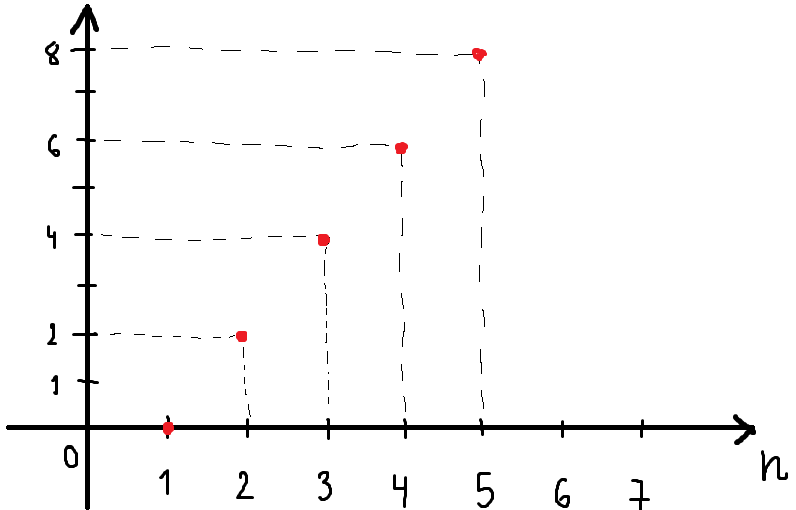
\includegraphics[width=0.5\textwidth]{slike/2n-2.png}
        \end{figure}
    \item Z rekurzivnim zapisom (s prejšnjimi členi): $ a_n = a_{n-1} + 2, a_1 = 0 $ (začetni pogoj) \didopomba{ne bo šlo pri vseh zaporedjih}
\end{itemize}

\vaje{
Vaje:
\begin{itemize}
    \item Zapis zaporedij iz splošnega člena, grafični prikaz
    \item Zapis splošnega člena iz zaporedja, iz grafičnega prikaza; zapis x-tega člena zaporedja
    \item uporabljaj različne črke, ne le $ a $
\end{itemize}
}

\end{priprava}